\documentclass[11pt,a4paper]{article}

% ---------- Layout ----------
\usepackage[margin=2.2cm,top=2.4cm,bottom=2.6cm]{geometry}
\usepackage[T1]{fontenc}
\usepackage[utf8]{inputenc}
\usepackage{helvet}
\renewcommand{\familydefault}{\sfdefault}
\usepackage{microtype}
\usepackage{parskip}
\usepackage{enumitem}
\usepackage{booktabs}
\usepackage{array}
\usepackage{longtable}
\usepackage{xcolor}
\usepackage{tikz}
\usetikzlibrary{shapes.geometric,arrows.meta,positioning,fit,backgrounds,calc}
\usepackage{tcolorbox}
\tcbuselibrary{skins,breakable}
\usepackage{fancyhdr}
\usepackage{titlesec}
\usepackage[hidelinks,colorlinks=false]{hyperref}
\usepackage{fontawesome5}
\usepackage{capt-of}
\usepackage{float}
\setlength{\headheight}{24pt}

% ---------- Palette ----------
\definecolor{navy}{HTML}{16324F}
\definecolor{steel}{HTML}{2E75B6}
\definecolor{teal}{HTML}{128A7D}
\definecolor{amber}{HTML}{C8790D}
\definecolor{purple}{HTML}{6C3483}
\definecolor{slate}{HTML}{5B6B79}
\definecolor{lightbg}{HTML}{F4F6F8}
\definecolor{hairline}{HTML}{D6DCE1}

\definecolor{phaseA}{HTML}{2E75B6} % ingestion - steel blue
\definecolor{phaseB}{HTML}{128A7D} % processing - teal
\definecolor{phaseC}{HTML}{C8790D} % storage - amber
\definecolor{phaseD}{HTML}{6C3483} % serving - purple

% ---------- Headings ----------
\titleformat{\section}
  {\Large\bfseries\color{navy}}{\thesection}{0.6em}{}[{\color{hairline}\titlerule[1pt]}]
\titleformat{\subsection}
  {\large\bfseries\color{steel}}{\thesubsection}{0.5em}{}
\titlespacing*{\section}{0pt}{22pt}{10pt}
\titlespacing*{\subsection}{0pt}{14pt}{6pt}

\pagestyle{fancy}
\fancyhf{}
\renewcommand{\headrulewidth}{0.6pt}
\renewcommand{\headrule}{\hbox to\headwidth{\color{hairline}\leaders\hrule height \headrulewidth\hfill}}
\lhead{\small\color{slate}AspiroBrain Data Pipeline --- Implementation Plan}
\rhead{\small\color{slate}AspiroEdu Internal}
\cfoot{\small\color{slate}\thepage\ of \pageref{LastPage}}
\usepackage{lastpage}

% ---------- Callout boxes ----------
\newtcolorbox{infobox}[1][]{
  breakable, enhanced, colback=steel!6, colframe=steel,
  boxrule=0.6pt, left=8pt, right=8pt, top=6pt, bottom=6pt,
  arc=2pt, title={#1}, fonttitle=\bfseries\small, coltitle=white,
  colbacktitle=steel
}
\newtcolorbox{actionbox}[1][]{
  breakable, enhanced, colback=teal!7, colframe=teal,
  boxrule=0.6pt, left=8pt, right=8pt, top=6pt, bottom=6pt,
  arc=2pt, title={#1}, fonttitle=\bfseries\small, coltitle=white,
  colbacktitle=teal
}
\newtcolorbox{riskbox}[1][]{
  breakable, enhanced, colback=amber!8, colframe=amber,
  boxrule=0.6pt, left=8pt, right=8pt, top=6pt, bottom=6pt,
  arc=2pt, title={#1}, fonttitle=\bfseries\small, coltitle=white,
  colbacktitle=amber
}

\newcolumntype{L}[1]{>{\raggedright\arraybackslash}p{#1}}

\begin{document}
\pagenumbering{gobble}

% ============================================================
% COVER PAGE
% ============================================================
\begin{titlepage}
\newgeometry{margin=0cm}
\begin{tikzpicture}[remember picture, overlay]
  \fill[navy] (current page.north west) rectangle ([yshift=-7.2cm]current page.north east);
  \fill[steel] (current page.north west) rectangle ([yshift=-0.18cm]current page.north east);
  \node[anchor=north west, text=white, font=\bfseries\Huge, align=left] at ([xshift=2.4cm,yshift=-3.0cm]current page.north west) {AspiroBrain};
  \node[anchor=north west, text=white!85!black, font=\Large, align=left] at ([xshift=2.4cm,yshift=-4.15cm]current page.north west) {Data Pipeline --- Implementation Plan};
  \node[anchor=north west, text=white!70!black, font=\normalsize, align=left] at ([xshift=2.4cm,yshift=-5.15cm]current page.north west) {From scraped CSVs to a trustworthy, hallucination-resistant data foundation};
  \draw[white!50!black, line width=0.6pt] ([xshift=2.4cm,yshift=-5.7cm]current page.north west) -- ([xshift=-2.4cm,yshift=-5.7cm]current page.north east);
  \node[anchor=north west, text=white!85!black, font=\small] at ([xshift=2.4cm,yshift=-6.15cm]current page.north west) {Prepared by Ahsanul Hoque \ $\vert$\ AspiroWork Data Internship \ $\vert$\ 10 July 2026};
\end{tikzpicture}

\vspace{8.4cm}

\begin{center}
\begin{minipage}{0.86\textwidth}
\begin{infobox}[Document Purpose]
This document translates the \emph{``Research Note: Data Challenges in Building AspiroBrain''} into a phased, engineering-ready implementation plan. It is grounded in the scraping pipeline already running today (Netherlands and Malta master's program data, 200 records, \texttt{mastersportal.com}), and proposes the concrete architecture, technology choices, and rollout sequence needed to turn that data into a foundation the AspiroBrain LLM assistant can trust.
\end{infobox}
\end{minipage}
\end{center}

\vfill
\begin{center}
\small\color{slate} Confidential --- Internal AspiroEdu Working Document
\end{center}
\vspace{1cm}
\restoregeometry
\end{titlepage}

\pagenumbering{arabic}
\setcounter{page}{2}

% ============================================================
\tableofcontents
\thispagestyle{fancy}
\newpage

% ============================================================
\section{Executive Summary}
% ============================================================

AspiroBrain's success depends less on the LLM than on the data feeding it. The research note identifies seven concrete failure modes --- wrong currency, inconsistent formats, silent gaps, stale data, duplicate programs, untrustworthy sources, and unmanageable scale --- each of which can translate directly into a student missing a deadline, misjudging a budget, or losing trust in the platform.

This plan proposes a four-phase build, each with an explicit trigger for moving to the next phase, so effort is never spent ahead of actual need:

\begin{itemize}[leftmargin=1.4em, itemsep=3pt]
  \item \textbf{Phase 0 --- Fix now.} Add three missing columns to the existing CSV pipeline. Half a day of work, removes the most expensive-to-backfill-later gaps.
  \item \textbf{Phase 1 --- Automate.} Turn manual scrape sessions into a scheduled, self-validating pipeline with change detection, so re-verification cost stops scaling linearly with catalog size.
  \item \textbf{Phase 2 --- Structure.} Replace the flat CSV with a relational data model that gives every program a stable identity and every fact a source, a trust tier, and a freshness timestamp.
  \item \textbf{Phase 3 --- Ground the LLM.} Wire AspiroBrain's retrieval and response generation so it can only state facts it actually retrieved, and is architecturally incapable of inventing a tuition figure or a deadline.
\end{itemize}

Phases 0--1 require no new infrastructure and can start immediately inside the current workflow. Phases 2--3 require an infrastructure and timeline decision from the team --- flagged explicitly in \S\ref{sec:open-questions}.

% ============================================================
\section{Problem Statement}
% ============================================================

The research note identifies seven data challenges. Table~\ref{tab:problems} maps each to its root cause and the concrete student-facing consequence if left unaddressed --- this is the ``why'' behind every architectural decision in \S\ref{sec:architecture}.

\begingroup
\renewcommand{\arraystretch}{1.35}
\begin{center}
\small
\begin{tabular}{@{}p{3.1cm}p{4.7cm}p{5.6cm}@{}}
\toprule
\textbf{Challenge} & \textbf{Root Cause} & \textbf{Student-Facing Risk} \\
\midrule
1. Multi-currency & Tuition published in EUR/GBP/USD/CAD/\dots; students think in BDT & Stored conversions go stale as FX rates move; budget looks wrong \\
2. Heterogeneous sources & Same fact phrased differently across sites (``Fall Intake'' vs ``Autumn Semester'') & Duplicate or missed results; poor search quality \\
3. Missing data & Universities publish fields gradually & LLM invents a plausible but false answer (hallucination) \\
4. Data freshness & Tuition/deadlines/requirements change yearly & Recommends an outdated fee or a passed deadline \\
5. Program identity & Universities rename/rebrand programs & Duplicate listings; broken continuity across re-scrapes \\
6. Source governance & Conflicting values across sources of unequal reliability & System has no basis to decide which number to trust \\
7. Scalability & Manual verification does not scale to hundreds of universities & Data quality degrades exactly as the catalog grows \\
\bottomrule
\end{tabular}
\captionof{table}{The seven data challenges, their cause, and their downstream risk.}
\label{tab:problems}
\end{center}
\endgroup

\begin{infobox}[Current State --- 10 July 2026]
Two country CSVs (Netherlands, Malta; 200 programs total), single source (\texttt{mastersportal.com} --- Tier 5 of 6 on the trust hierarchy in \S\ref{sec:governance}). Known schema gaps: no \texttt{currency} column, no \texttt{last\_verified\_date}, no \texttt{program\_id}; repeatable fields flattened into semicolon-separated text. Two real bugs already caught and fixed by hand during scraping: \emph{tuition front-loading} (headline ``\texteuro X/year'' is sometimes an average across an uneven multi-year fee schedule) and \emph{scholarship-widget noise} (a sitewide generic scholarship list bleeding into program-specific tags).
\end{infobox}

% ============================================================
\section{Solution Architecture}
\label{sec:architecture}
% ============================================================

Figure~\ref{fig:architecture} shows the full pipeline as four layers, each corresponding to one implementation phase. Data flows top to bottom: raw pages are scraped and frozen, then cleaned and quality-checked, then loaded into a structured store with identity and trust metadata, then served to the LLM through an API that enforces freshness and handles currency conversion live.

\begin{figure}[H]
\centering
\resizebox{\textwidth}{!}{%
\begin{tikzpicture}[
  node distance=1.0cm and 1.0cm,
  every node/.style={font=\small},
  box/.style={rectangle, rounded corners=3pt, draw, thick, align=center,
              minimum height=1.25cm, text width=3.05cm, inner sep=5pt},
  arr/.style={-{Latex[length=2.8mm,width=2mm]}, thick}
]

% ---- Row A: Ingestion ----
\node[box, fill=phaseA!12, draw=phaseA] (A1) {\textbf{Scrape}\\[1pt]\footnotesize WebFetch + defuddle};
\node[box, fill=phaseA!12, draw=phaseA, right=1.1cm of A1] (A2) {\textbf{Bronze Snapshots}\\[1pt]\footnotesize immutable, timestamped};
\draw[arr, phaseA] (A1) -- (A2);

% ---- Row B: Processing & Quality ----
\node[box, fill=phaseB!12, draw=phaseB, below=2.55cm of A1, xshift=-0.05cm] (B1) {\textbf{Normalize}\\[1pt]\footnotesize lookup table + RapidFuzz};
\node[box, fill=phaseB!12, draw=phaseB, right=1.1cm of B1] (B2) {\textbf{Validate}\\[1pt]\footnotesize Pandera schema check};
\node[box, fill=phaseB!12, draw=phaseB, right=1.1cm of B2] (B3) {\textbf{Diff}\\[1pt]\footnotesize hash vs.\ last snapshot};
\node[box, fill=phaseB!12, draw=phaseB, right=1.1cm of B3] (B4) {\textbf{Entity Resolution}\\[1pt]\footnotesize exact $\to$ fuzzy $\to$ embedding};
\draw[arr, phaseB] (B1) -- (B2);
\draw[arr, phaseB] (B2) -- (B3);
\draw[arr, phaseB] (B3) -- (B4);
\draw[arr, slate] (A2.south) to[out=-90,in=90] (B1.north);

% ---- Row C: Storage ----
\node[box, fill=phaseC!12, draw=phaseC, below=2.55cm of B2, xshift=1.6cm, text width=6.6cm, minimum height=1.4cm] (C1)
  {\textbf{Relational Store}\\[1pt]\footnotesize SQLite now $\to$ Postgres / Supabase later\\[1pt]\footnotesize university $\cdot$ program $\cdot$ fee\_line $\cdot$ intake $\cdot$ requirement};

\draw[arr, slate] (B4.south) to[out=-90,in=90] (C1.north);

% ---- Row D: Serving ----
\node[box, fill=phaseD!12, draw=phaseD, below=2.55cm of C1, xshift=-1.75cm] (D1) {\textbf{Access API}\\[1pt]\footnotesize filtered queries + live FX};
\node[box, fill=phaseD!12, draw=phaseD, right=1.1cm of D1, text width=3.4cm] (D2) {\textbf{AspiroBrain LLM}\\[1pt]\footnotesize tool-calling, field-level grounding};
\draw[arr, phaseD] (D1) -- (D2);
\draw[arr, slate] (C1.south) to[out=-90,in=90] (D1.north);

% ---- Background phase bands ----
\begin{pgfonlayer}{background}
\node[fit=(A1)(A2), fill=phaseA!5, draw=phaseA!55, rounded corners=9pt, inner sep=11pt] (bandA) {};
\node[fit=(B1)(B2)(B3)(B4), fill=phaseB!5, draw=phaseB!55, rounded corners=9pt, inner sep=11pt] (bandB) {};
\node[fit=(C1), fill=phaseC!5, draw=phaseC!55, rounded corners=9pt, inner sep=11pt] (bandC) {};
\node[fit=(D1)(D2), fill=phaseD!5, draw=phaseD!55, rounded corners=9pt, inner sep=11pt] (bandD) {};
\end{pgfonlayer}

\node[anchor=south west, text=phaseA, font=\bfseries\footnotesize] at ([yshift=3pt]bandA.north west) {PHASE 0--1 \ $\bullet$ \ INGESTION};
\node[anchor=south west, text=phaseB, font=\bfseries\footnotesize] at ([yshift=3pt]bandB.north west) {PHASE 1 \ $\bullet$ \ PROCESSING \& QUALITY};
\node[anchor=south west, text=phaseC, font=\bfseries\footnotesize] at ([yshift=3pt]bandC.north west) {PHASE 2 \ $\bullet$ \ STORAGE};
\node[anchor=south west, text=phaseD, font=\bfseries\footnotesize] at ([yshift=3pt]bandD.north west) {PHASE 3 \ $\bullet$ \ SERVING};

\end{tikzpicture}%
}
\caption{AspiroBrain data pipeline: four layers, each mapped to an implementation phase. Every arrow closes at least one of the seven challenges in Table~\ref{tab:problems} --- normalization resolves heterogeneous formats, the diff step resolves freshness, entity resolution resolves program identity, and the storage layer's trust-tier and verification fields feed directly into how the LLM is allowed to answer.}
\label{fig:architecture}
\end{figure}

\subsection{Why hybrid retrieval, not vector-search-everywhere}
Structured questions (country, budget, degree level, deadline) are answered with a direct filtered query against the relational store --- no embeddings involved, no risk of a vector search silently dropping a hard constraint like budget. Fuzzy-intent questions (``I want to work in robotics'') are embedded, matched against candidate programs via vector similarity, and then the same hard filters are re-applied via SQL before anything reaches the student. Vectors generate candidates; they never enforce a constraint.

\subsection{Why tool-calling is the primary hallucination defense}
\label{sec:grounding}
The LLM never free-generates a fact. It calls \texttt{get\_program\_details(program\_id)}, which returns typed JSON where every field carries its own \texttt{value}, \texttt{verification\_status}, and \texttt{last\_verified\_date}. The system prompt requires the model to state only values present in that tool output, and to emit an explicit fallback --- \emph{``could not be verified from official university sources, please consult an Aspiro counselor''} --- whenever a field is null or unverified. A cheap post-generation check (flag any number or date absent from the tool payload) is a secondary net, not the primary defense.

% ============================================================
\section{Phased Roadmap}
% ============================================================

\begingroup
\renewcommand{\arraystretch}{1.5}
\small
\begin{longtable}{@{}L{1.6cm}L{2.7cm}L{5.0cm}L{4.3cm}@{}}
\caption{Four-phase rollout. Phases 0--1 require no new infrastructure; Phases 2--3 need a team infrastructure decision (see \S\ref{sec:open-questions}).}\\
\toprule
\textbf{Phase} & \textbf{Timeframe} & \textbf{Key Deliverables} & \textbf{Exit Trigger (move to next phase)} \\
\midrule
\endfirsthead
\multicolumn{4}{@{}l}{\small\itshape Table 2 continued} \\
\toprule
\textbf{Phase} & \textbf{Timeframe} & \textbf{Key Deliverables} & \textbf{Exit Trigger (move to next phase)} \\
\midrule
\endhead
\bottomrule
\endfoot
\bottomrule
\endlastfoot
\textbf{0 --- Fix Now} & Immediate, $<$1 day & Add \texttt{currency}, \texttt{last\_verified\_date}, \texttt{program\_id} columns; freeze existing CSVs as immutable Bronze snapshots & Done as soon as the columns are backfilled --- no dependency \\
\textbf{1 --- Automate} & 2--4 weeks & Cron-scheduled scraping; SHA-256 change detection; 3-tier normalization (lookup $\to$ RapidFuzz $\to$ LLM); Pandera validation; live FX via free API & Catalog passes $\sim$5 countries \emph{or} manual re-verification becomes the bottleneck \\
\textbf{2 --- Structure} & Follows Phase 1 & Relational schema live in SQLite; 3-stage entity resolution; thin access API with freshness/trust filtering & Concurrent writers appear, \emph{or} row count approaches 50k, \emph{or} the LLM backend needs networked (non-embedded) access \\
\textbf{3 --- Ground the LLM} & Parallel with / after Phase 2 & Hybrid retrieval (SQL + pgvector); tool-calling grounding; deterministic FX tool calls; trust-tier disclosure in responses & Production launch readiness \\
\end{longtable}
\endgroup

% ============================================================
\section{Data Model}
% ============================================================

Phase 2 replaces the flat 17-column CSV with a normalized schema. Repeatable fields (prerequisites, tags, intakes) become real child rows instead of semicolon-flattened text, and every fact-bearing table carries its own source, trust tier, and verification status --- freshness and governance are schema properties, not an afterthought.

\begin{center}
\small
\begin{tabular}{@{}L{2.6cm}L{9.9cm}@{}}
\toprule
\textbf{Table} & \textbf{Purpose \& Key Fields} \\
\midrule
\texttt{university} & One row per institution: name, country, city, website, \texttt{source\_tier}. \\
\texttt{program} & Canonical program record: level, field, duration, \texttt{last\_verified\_date}, \texttt{verification\_status}, \texttt{confidence\_level}, \texttt{superseded\_by}. \\
\texttt{program\_alias} & Every scraped title variant ever seen for a program --- the join point for entity resolution and the audit trail. \\
\texttt{fee\_line} & One row per fee (tuition year 1, tuition total, application fee, deposit) in its \textbf{original currency}, never pre-converted. \\
\texttt{intake} & One row per intake term/deadline, with \texttt{term\_normalized} mapped through the controlled vocabulary. \\
\texttt{requirement} & One row per prerequisite/must-have, with \texttt{is\_confirmed\_absent} distinguishing ``checked, none exist'' from ``not yet checked.'' \\
\texttt{tag} / \texttt{program\_tag} & Scholarships, campus features, accreditations --- many-to-many, filtered clean of sitewide noise. \\
\texttt{source} / \texttt{term\_dictionary} & Source registry with trust tier; growing lookup table that powers the normalization layer. \\
\bottomrule
\end{tabular}
\end{center}

\subsection{Program identity resolution}
Three stages, cheapest first, so most rows never need the expensive path:
\begin{enumerate}[leftmargin=1.6em, itemsep=2pt]
  \item \textbf{Exact match} on normalized \texttt{(university, program name)} --- auto-updates the existing record.
  \item \textbf{Fuzzy match} via RapidFuzz --- $\geq 0.95$ similarity auto-merges; $0.85$--$0.95$ is flagged for a short human review queue; below $0.85$ is treated as a new program.
  \item \textbf{Embedding similarity} --- used only as a tiebreaker signal inside the flagged band, not as an auto-merge trigger. Deferred until catalog volume actually justifies the cost.
\end{enumerate}

% ============================================================
\section{Source Governance}
\label{sec:governance}
% ============================================================

Every fact carries a numeric \texttt{source\_tier}, stored \emph{per record} (not just per university) so that a future Tier-1 fee line can outrank an existing Tier-5 line for the same program the moment it appears.

\begin{center}
\small
\begin{tabular}{@{}cL{9.6cm}@{}}
\toprule
\textbf{Tier} & \textbf{Source Type} \\
\midrule
1 & Official university website \\
2 & Official university API \\
3 & Partner institution portal \\
4 & Internal, human-verified Aspiro records \\
5 & Third-party aggregator \emph{(mastersportal.com --- 100\% of current data)} \\
6 & User-generated content \\
\bottomrule
\end{tabular}
\end{center}

\begin{riskbox}[Honest Flag]
Every record collected to date sits at Tier 5. The governance machinery above only pays off once a second, higher-trust source enters the pipeline --- until then, AspiroBrain has no conflicting values to arbitrate between, only a single (unverified-by-the-university) source to lean on. See Open Question 1 below.
\end{riskbox}

% ============================================================
\section{Technology Stack}
% ============================================================

\begingroup
\renewcommand{\arraystretch}{1.4}
\begin{center}
\small
\begin{tabular}{@{}L{2.5cm}L{3.3cm}L{3.6cm}L{3.2cm}@{}}
\toprule
\textbf{Layer} & \textbf{Now} & \textbf{Upgrade Trigger} & \textbf{Later} \\
\midrule
Orchestration & cron + Python scripts & $>$5 countries, or retries/alerting needed & Prefect OSS \\
Normalization & static lookup + RapidFuzz & unresolved-phrase volume grows & + LLM fallback, written back to lookup table \\
Validation & Pandera & multi-engine pipelines, non-technical stakeholders & Great Expectations \\
Storage & SQLite + Litestream & concurrent writers, $\sim$50k+ rows, network access needed & Supabase (Postgres) \\
Entity resolution & exact $\to$ RapidFuzz & review queue too large for manual handling & + embedding tiebreaker \\
Vector search & none & fuzzy-intent queries go live & pgvector, same Postgres instance \\
FX rates & Frankfurter API (primary), fawazahmed0 (fallback) & intraday-rate need & Paid tier (ExchangeRate-API, Open Exchange Rates) \\
LLM grounding & --- & --- & Tool-calling, field-level grounding (\S\ref{sec:grounding}) \\
\bottomrule
\end{tabular}
\captionof{table}{Every layer has a stated upgrade trigger --- nothing here is over-built for a 200-row catalog run by one intern.}
\end{center}
\endgroup

% ============================================================
\section{Open Questions for the Team}
\label{sec:open-questions}
% ============================================================

\begin{riskbox}[Decisions Needed Before Phase 2--3]
\begin{enumerate}[leftmargin=1.6em, itemsep=4pt]
  \item Is \texttt{mastersportal.com} meant to remain the sole data source, or is there a plan to reach Tier-1/Tier-2 sources? The trust-hierarchy design only earns its keep once more than one tier is actually represented in the data.
  \item Who owns the fuzzy-match review queue (the $0.85$--$0.95$ band) and flagged data changes --- the intern, a counselor, or does this need a lightweight review UI?
  \item What is the realistic timeline and budget for standing up Postgres/Supabase and an LLM backend? Phases 0--1 run entirely inside the current CSV/git workflow; Phases 2--3 need an infrastructure decision from the team.
\end{enumerate}
\end{riskbox}

% ============================================================
\section{Recommended Immediate Action}
% ============================================================

\begin{actionbox}[Next Step --- No Infrastructure Required]
Phase 0 can be completed today inside the existing \texttt{Data Collection/} workflow: add \texttt{currency}, \texttt{last\_verified\_date}, and \texttt{program\_id} columns, and freeze the current Netherlands and Malta CSVs as immutable Bronze snapshots. This is roughly half a day of work and removes the schema gaps that get exponentially more expensive to backfill once the catalog grows past a handful of countries.
\end{actionbox}

\vspace{0.6cm}
{\small\color{slate}\textit{Prepared as part of the AspiroWork data internship, grounded in the live mastersportal.com scraping pipeline (Netherlands + Malta, 200 programs, 10 July 2026). Full research citations available on request.}}

\end{document}
